\documentclass{article}

\usepackage{tikz, hyperref, cleveref, apacite, graphicx, caption, subcaption, listings}
\usepackage[inkscapeformat=png]{svg}
\crefname{lstlisting}{listato}{listings}
\Crefname{lstlisting}{Listato}{Listings}

\crefformat{section}{\S#2#1#3}
\crefformat{subsection}{\S#2#1#3}
\crefformat{subsubsection}{\S#2#1#3}
\crefformat{figure}{#2Figura~#1#3}
\crefformat{footnote}{#2\footnotemark[#1]#3}
\crefformat{table}{#2Tabella~#1#3}

\usepackage[bottom]{footmisc}
\usepackage[margin=1in]{geometry}
\renewcommand{\contentsname}{Indice}
\renewcommand{\refname}{Riferimenti}

\lstset{
  language=C,                % choose the language of the code
  numbers=left,                   % where to put the line-numbers
  stepnumber=1,                   % the step between two line-numbers.        
  numbersep=5pt,                  % how far the line-numbers are from the code
  backgroundcolor=\color{white},  % choose the background color. You must add \usepackage{color}
  showspaces=false,               % show spaces adding particular underscores
  showstringspaces=false,         % underline spaces within strings
  showtabs=false,                 % show tabs within strings adding particular underscores
  tabsize=2,                      % sets default tabsize to 2 spaces
  captionpos=b,                   % sets the caption-position to bottom
  breaklines=true,                % sets automatic line breaking
  breakatwhitespace=true,         % sets if automatic breaks should only happen at whitespace
  title=\lstname,                 % show the filename of files included with \lstinputlisting;
}

\author{Giuseppe Capasso}

\begin{document}

\begin{titlepage}
  \thispagestyle{empty}
  \raggedright % Allinea a sinistra

  \begin{tikzpicture}
    \node[anchor=south west] at (4,0) {
\includegraphics[scale=0.75]{./figures/unina-logo-1.png}};
    \node[anchor=south west] at (0,1.5) {
\includegraphics{./figures/unina-logo-2.png}};
    \node[anchor=south west] at (0,0.5) {\textsf{Scuola Politecnica e delle Scienze di Base}};
    \node[anchor=south west] at (0,0) {\textsf{Corso di Laurea Magistrale in Ingegneria Informatica}};
  \end{tikzpicture}

  \vfill

  {\textbf{\textit{\LARGE Fuzzing Linux IPsec implementation with Syzkaller}}}
  \\[2cm]

  {\textbf{\textit{\Large Progetto di Software Security}}}
  \\[1cm]
  {\large Anno Accademico 2023/2024}

  \vfill

  \begin{table}[h]
    \textbf{Giuseppe Capasso}
    \\
    \textbf{matr. M63001498}
  \end{table}

\end{titlepage}

\tableofcontents
\newpage

\section*{Introduzione}
Negli ultimi anni, il kernel Linux ha visto un aumento significativo nell'adozione del
fuzzing come strumento di sicurezza. Progetti come Syzkaller, sviluppato da Google, 
hanno dimostrato l'efficacia di questa tecnica nel rilevare numerose vulnerabilità prima
che possano essere sfruttate da attori malintenzionati. Syzkaller utilizza tecniche
avanzate per generare input complessi e coprire ampie porzioni del codice del kernel,
identificando bug che potrebbero rimanere nascosti ai metodi di testing tradizionali.

Lo scopo del progetto è quello di esplorare l'attività di fuzzing per la ricerca di bug e 
vulnerabilità nel kernel Linux. Il kernel Linux è un'applicazione monolitic, concorrente e 
asincrona che prende direttamente il controllo dell'hardware il cui fallimento (detto \textbf{\textit{kernel panic}})
porta il sistema in \textit{crash} permanente. 

Il kernel Linux è composto da diversi sottosistemi ciascuno dei quali espone un'interfaccia 
verso l'utente che può essere utilizzata per il fuzzing congiuntamente allo sviluppo degli 
strumenti per l'analisi per \\
l'individuazione di bug in memoria a \textit{runtime}
quali \textbf{\textit{KASAN}} (utilizzato come \textit{address sanitizer}), 
\textbf{\textit{KMSAN}} (utilizzato come memory sanitizer), il più recente
\textbf{\textit{KCMSAN}} (utilizzato per individuare \textit{race condition}) e 
all'introduzione dell'opzione \textbf{\textit{KCOV}} per l'instrumentazione del codice 
kernel.

\clearpage

\section{Fuzzing}
Il fuzzing è una tecnica utilizzata per effettuare testing di robustezza e sicurezza delle 
applicazioni basata sulla generazione automatica di input. I fuzzer possono essere 
classificati in:
\begin{itemize}
  \item puramente randomici: producono per la maggior parte input non validi;
  \item generativi: si basano su modelli (come FSM) dei protocolli e cercano di navigarli
    per generare input validi;
  \item basati su mutazione: partono da \textbf{\textit{seed}} validi e mutano il seeed 
    per generare altri input;
\end{itemize}

Il kernel Linux è un'applicazione monolitica, concorrente ed asincrona che espone un'interfaccia
verso gli utenti sottoforma di system-call. Il fuzzing di quest'applicazione richiede
l'utilizzo di strumenti per individuare bug nell'utilizzo della memoria. In particolare, 
sono stati abilitati:
\begin{itemize}
  \item KASAN: strumento di debug per il kernel Linux progettato per rilevare errori di
    memoria come buffer overflow, use-after-free e altri tipi di violazioni di accesso
    alla memoria. Utilizza un meccanismo basato su shadow memory per monitorare le 
    allocazioni e le deallocazioni di memoria, segnalandosi quando si verificano accessi
    illegali (\cref{fig:kasan} e 
    \cref{fig:kasan-shadow}). Inoltre,
    KASAN introduce il concetto di \textbf{\textit{quarantine}} che viene utilizzato 
    per evitare gli errori \textbf{\textit{use-after-free}} nello \textit{heap} che 
    altrimenti sarebbe gestito con una politica LIFO dal kernel (\cref{fig:kasan-quarantine} e 
    \cref{fig:kasan-quarantine-2});
  \item KMSAN: strumento di debug utilizzato per individuare valori di memoria non 
    inizializzati. Analogamente, al caso KASAN, utilizza gli shadow byte per tenere traccia 
    della memoria allocata;
\end{itemize}

\begin{figure}[h]
  \begin{center}
    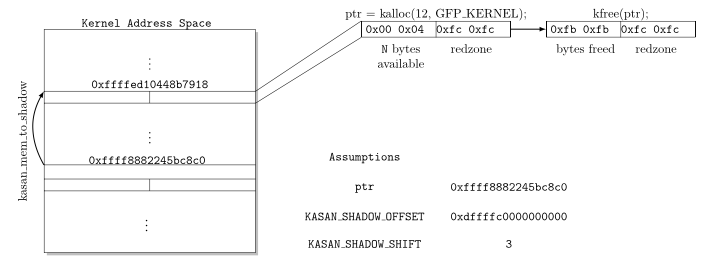
\includegraphics[width=0.95\textwidth]{figures/kasan.png}
  \end{center}
  \caption{Allocazione di un range di indirizzi nel kernel}\label{fig:kasan}
\end{figure}

\begin{figure}[h]
  \begin{center}
    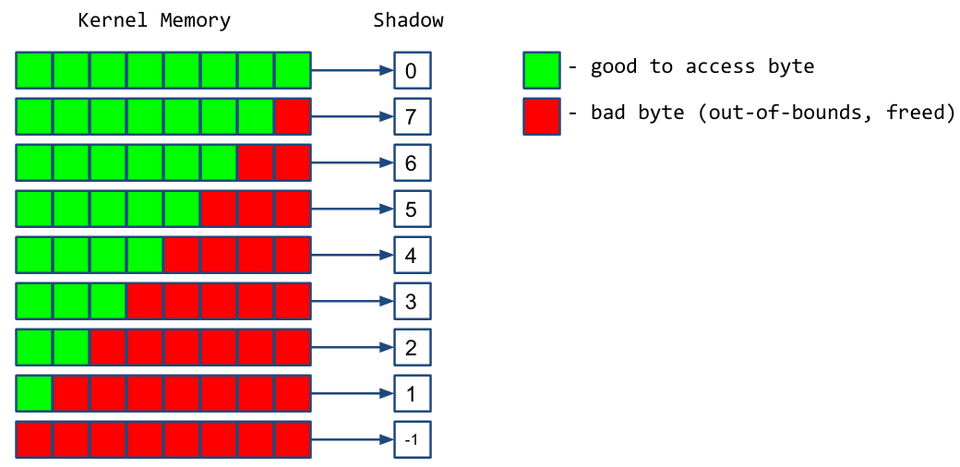
\includegraphics[width=0.95\textwidth]{figures/kasan-shadow.png}
  \end{center}
  \caption{Shadow byte per controllare le allocazioni}\label{fig:kasan-shadow}
\end{figure}


\begin{figure}[h]
  \begin{center}
    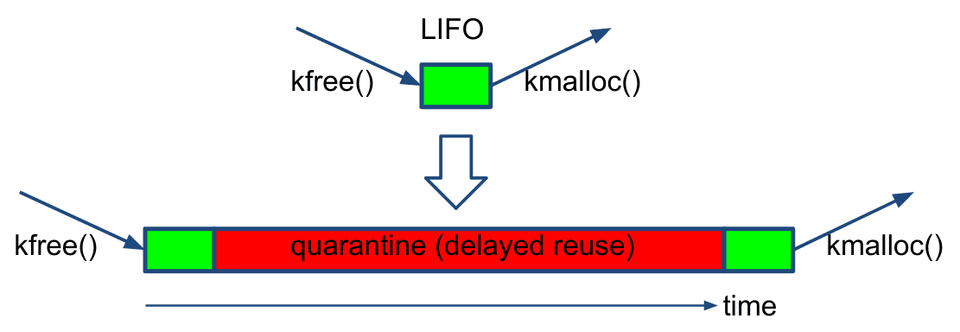
\includegraphics[width=.7\textwidth]{figures/kasan-quarantine.png}
  \end{center}
  \caption{Kasan quarantena per gli oggetti dell'heap}\label{fig:kasan-quarantine}
\end{figure}

\begin{figure}[h]
  \begin{center}
    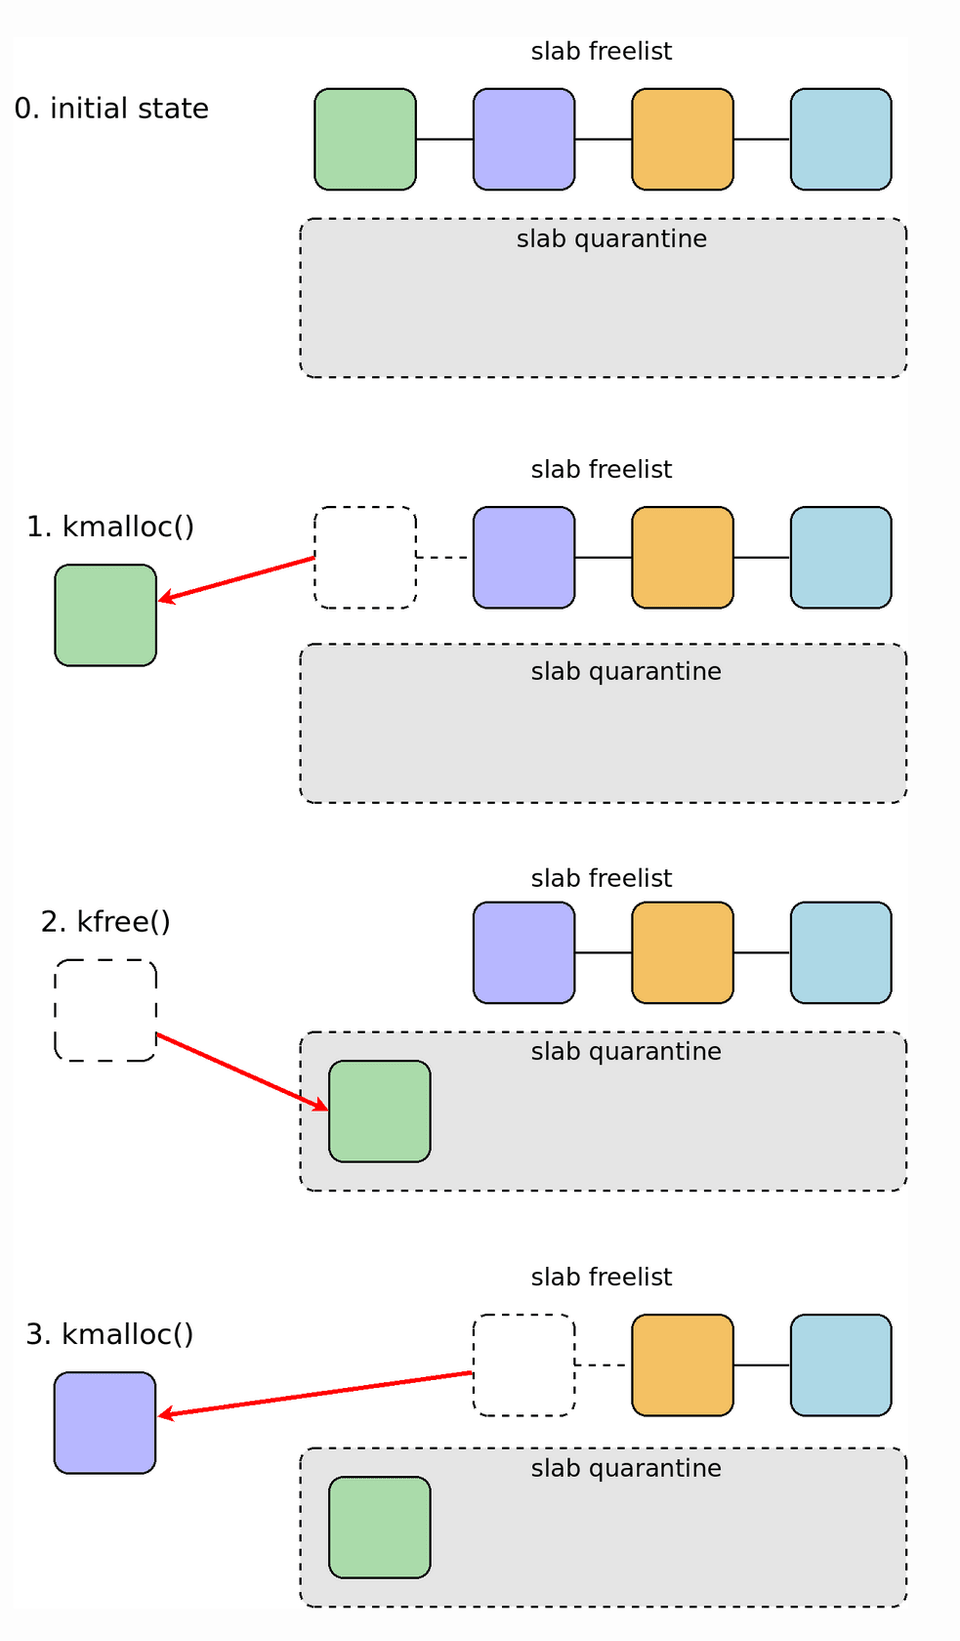
\includegraphics[width=.7\textwidth]{figures/kasan-quarantine-2.png}
  \end{center}
  \caption{Use-after-free con KASAN}\label{fig:kasan-quarantine-2}
\end{figure}



\subsection{Syzkaller}
Syzkaller\cite{Syzkaller} è un'applicazione che effettua \textbf{\textit{generative fuzzing}} di applicazioni 
kernel in ambiente virtualizzato il cui "seed" è un programma che consiste in una sequenza di system-call. 
La tecnica utilizzata è detta \textbf{\textit{coverage-based}}: decide che un programma ha 
un'altra probabilità di sopravvivere nella generazione di input in base alla copertura 
che offre.

Con riferimento al kernel Linux, l'input è costituito da 
system-call descritte staticamente attraverso \textbf{\textit{syzlang}} (un linguaggio 
dichiarativo) in semplici file di testo. Una sequenza di system-call forma un programma 
che può essere eseguito dal kernel e viene utilizzato da syzkaller per mutare e generare altri 
programmi. Ad esempio, un semplice programma che apre un file e legge alcuni byte da esso 
può essere scritto nel seguente modo \cite{Syzkaller}[docs/syscall\_descriptions.md]:

\begin{verbatim}
open(file filename, flags flags[open_flags], mode flags[open_mode]) fd
read(fd fd, buf buffer[out], count len[buf])
close(fd fd)
open_mode = S_IRUSR, S_IWUSR, S_IXUSR, S_IRGRP, S_IWGRP, S_IXGRP, S_IROTH, S_IWOTH, S_IXOTH
\end{verbatim}

Syzkaller ha la struttura modulare presentata in \cref{fig:syzkaller-arch}. 

\begin{figure}[h]
  \begin{center}
    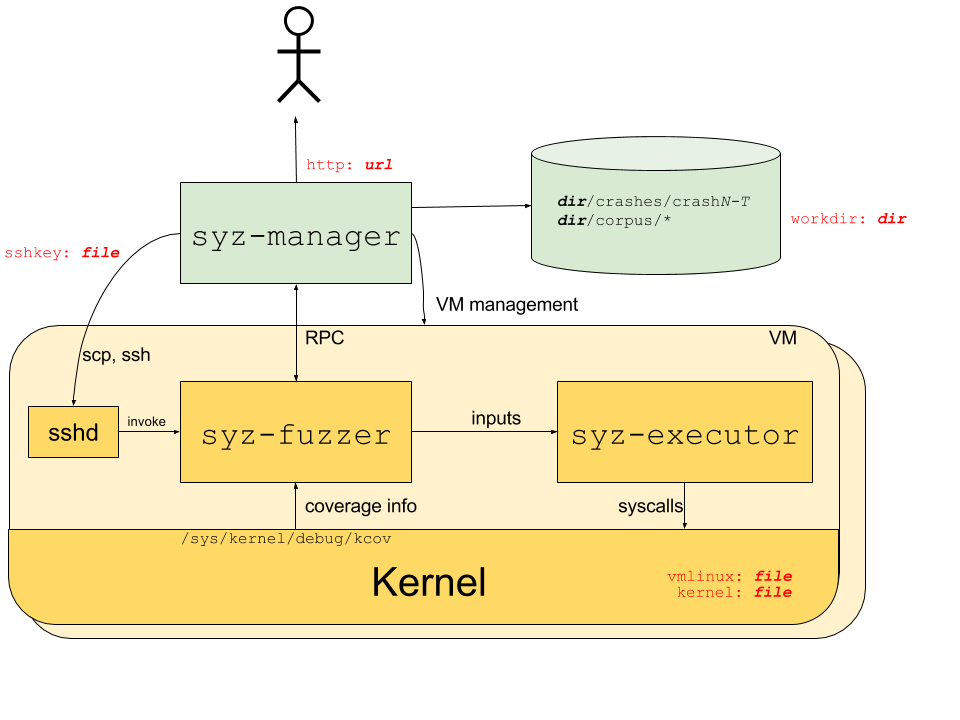
\includegraphics[width=.75\textwidth]{figures/process_structure.png}
  \end{center}
  \caption{Architettura Syzkaller}\label{fig:syzkaller-arch}
\end{figure}

\paragraph{Syz-manager}Syz-manager è il componente centrale di Syzkaller, responsabile della
gestione e del coordinamento dell'intero processo di fuzzing. Gestisce le configurazioni dei
test, avvia e controlla le istanze di Syz-fuzzer e monitora i risultati del fuzzing. 
Syz-manager raccoglie le statistiche, analizza i crash e mantiene un registro delle 
esecuzioni, facilitando il monitoraggio e l'analisi dei risultati. In particolare, si 
connette alla macchina target attraverso SSH, comunica con \textbf{\textit{syz-fuzzer}}.
Inoltre, syz-manager offre una dashboard di monitoraggio in cui si può verificare lo stato 
dell'esecuzione e analizzare eventuali crash riportati. 

\paragraph{Syz-fuzzer} Si occupa di generare input a partire dai programmi (collezionati 
in un corpus) proveniente dal manager. Inoltre, si occupa di monitorare lo stato del kernel 
cercando dei crash che si possono verificare per:
\begin{itemize}
  \item nessun output dalla macchina target;
  \item connessione alla macchina virtuale persa;
  \item macchina virtuale target non esegue nessun programma per molto tempo;
\end{itemize}
Infine, il fuzzer raccoglie metriche di coverage (grazie alla funzionalità KCOV) e le 
riporta attraverso un'API RPC al manager che fornisce un nuovo input.

\paragraph{Syz-executor} Si occupa di eseguire una sequenza di system-call che rieceve in 
ingresso dal fuzzer e comunica con il fuzzer attraverso una memoria condivisa.

\subsubsection{Syzlang}
Il linguaggio permette di definire \textbf{\textit{risorse}} che possono essere utilizzate 
come tipo di variabile e possono guidare il fuzzer durante la generazione di parametri di 
input. Ad esempio, la risorsa \textbf{\textit{filename}} indica al fuzzer di generare solo 
percorsi e nome di file validi in Linux. 

Alla descrizione formale delle system-call viene poi associato un programma che syzkaller 
può mostrare in:
\begin{itemize}
  \item binaria: caricato ed eseguito direttamente dal kernel;
  \item testuale: utilizzato per analizzare visivamente l'output del fuzzer;
  \item in codice C: syzkaller è in grado di generare un programma C da una rappresentazione
    binaria per essere d'aiuto agli sviluppatori nella riproduzione di bug e vulnerabilità 
    trovate;
\end{itemize}

Ad esempio, il programma descritto in precedenza può portare alla generazione del codice 
seguente con parametri reali:

\begin{verbatim}
r0 = open(&(0x7f0000000000)="./file0", 0x3, 0x9)
read(r0, &(0x7f0000000000), 42)
close(r0) 
\end{verbatim}

Inoltre, il linguaggio permette di definire costanti, campi di lunghezza variabile e 
\textbf{\textit{unions}}. Ad esempio, il seguente codice definisce il tipo \textbf{\textit{port\_sock}} 
come un intero $16$-bit che può andare da $20000$ a $20004$: 

\begin{verbatim}
type sock_port int16be[20000:20004] 
\end{verbatim}

Mentre, la seguente \textbf{\textit{union}} rappresenta alcuni indirizzi IPv4:

\begin{verbatim}
ipv4_addr [
# Random public addresses 100.1.1.[0-2]:
	rand_addr	int32be[0x64010100:0x64010102]
# 0.0.0.0:
	empty		const[0x0, int32be]
# 127.0.0.1:
	loopback	const[0x7f000001, int32be]
] [size[4]]
\end{verbatim}

Inoltre, in seguito viene dichiarato il \textbf{\textit{file descriptor}} di una \textit{socket}
ereditando dalla risorsa \textbf{\textit{fd}}\cite{SyzkallerExternalNetworking}:

\begin{verbatim}
resource sock[fd]
resource sock_in[sock]
resource sock_tcp[sock_in]
\end{verbatim}

Infine, le system-call descritte possono avere diverse varianti in base al tipo di configurazione 
ricevuta. Ad esempio, una socket UDP è diversa da una socket TCP, ma vengono generate a 
partire dalla stessa system-call. In syzlang, è possibile utilizzare il simbolo "\$" per 
indicare una versione particolare di una funzione\cite{SyzkallerExternalNetworking}:
\begin{verbatim}
socket$inet_tcp(domain const[AF_INET], type const[SOCK_STREAM],
                proto const[0]) sock_tcp
socket$inet_udp(domain const[AF_INET], type const[SOCK_DGRAM],
                proto const[0]) sock_udp

\end{verbatim}

\paragraph{Pseudo-system call} Syzlang consente di descrivere funzioni che non hanno una 
diretta implementazione nel kernel, ma può essere fornita dall'utente. Queste pseudo-syscall 
servono a configurare o a racchiudere in una sola funzione più system call. Ad esempio, 
per arrivare a testare il codice di rete è necessario fornire al fuzzer la nozione di 
connessione TCP che viene implementata attraverso la pseudo-syscall 
\textbf{\textit{syz\_emit\_ethernet}}.

\begin{verbatim}
syz_emit_ethernet(len len[packet], 
  packet ptr[in, eth_packet], 
  frags ptr[in, vnet_fragmentation, opt])
\end{verbatim}

\subsection{Esecuzione}
Una volta compilato syzkaller, è necessario:
\begin{itemize}
  \item compilare un kernel abilitando gli strumenti di coverage, debug e i sottosistemi
    che si vogliono testare;
  \item creare un'immagine "bootable" con programmi base della suite GNU;
\end{itemize}

\subsubsection{Preparazione del kernel}
I flag principali per instrumentare il codice del kernel sono i seguenti:
\begin{verbatim}
# Coverage collection.
CONFIG_KCOV=y

# Debug info for symbolization.
CONFIG_DEBUG_INFO=y

# Memory bug detector
CONFIG_KASAN=y
CONFIG_KASAN_INLINE=y

# Required for Debian Stretch
CONFIG_CONFIGFS_FS=y
CONFIG_SECURITYFS=y
\end{verbatim}
Una volta compilato il kernel, bisogna configurare l'immagine. In particolare, syzkaller 
fornisce uno script di configurazione in cui crea un'immagine debian a partire da un 
\textbf{\textit{rootfs}}.
In questa immagine sarà configurato opportunamente un server SSH 
e generata una coppia di chiavi per fornire l'accesso a syzkaller-manager. Una volta 
preparata l'immagine può essere effettuato il test con QEMU eseguendo il seguente comando: 


\begin{verbatim}
qemu-system-x86_64 \
	-m 2G \
	-smp 2 \
	-kernel $KERNEL/arch/x86/boot/bzImage \
	-append "console=ttyS0 root=/dev/sda earlyprintk=serial net.ifnames=0" \
	-drive file=$IMAGE/buster.img,format=raw \
	-net user,host=10.0.2.10,hostfwd=tcp:127.0.0.1:10021-:22 \
	-net nic,model=e1000 \
	-enable-kvm \
	-nographic \
	-pidfile vm.pid \
	2>&1 | tee vm.log   
\end{verbatim}

Infine, è possibile eseguire syzkaller con il seguente file di configurazione in cui si 
eseguono $8$ kernel in parallelo ciascuno con una cpu e in $1$GB di memoria e monitorare
il processo nella dashboard web \cref{fig:syz-dashboard}.
\begin{verbatim}
{
  "target": "linux/amd64",
  "http": "127.0.0.1:56741",
  "workdir": ""syzkaller/workdir",
  "kernel_obj": "$KERNEL",
  "image": "$IMAGE/buster.img",
  "sshkey": "$IMAGE/buster.id_rsa",
  "syzkaller": "syzkaller/",
  "procs": 8,
  "type": "qemu",
  "vm": {
    "count": 8,
    "kernel": "$KERNEL/arch/x86/boot/bzImage",
    "cpu": 1,
    "mem": 1024
  }
} 
\end{verbatim}

\begin{figure}[h]
  \begin{center}
    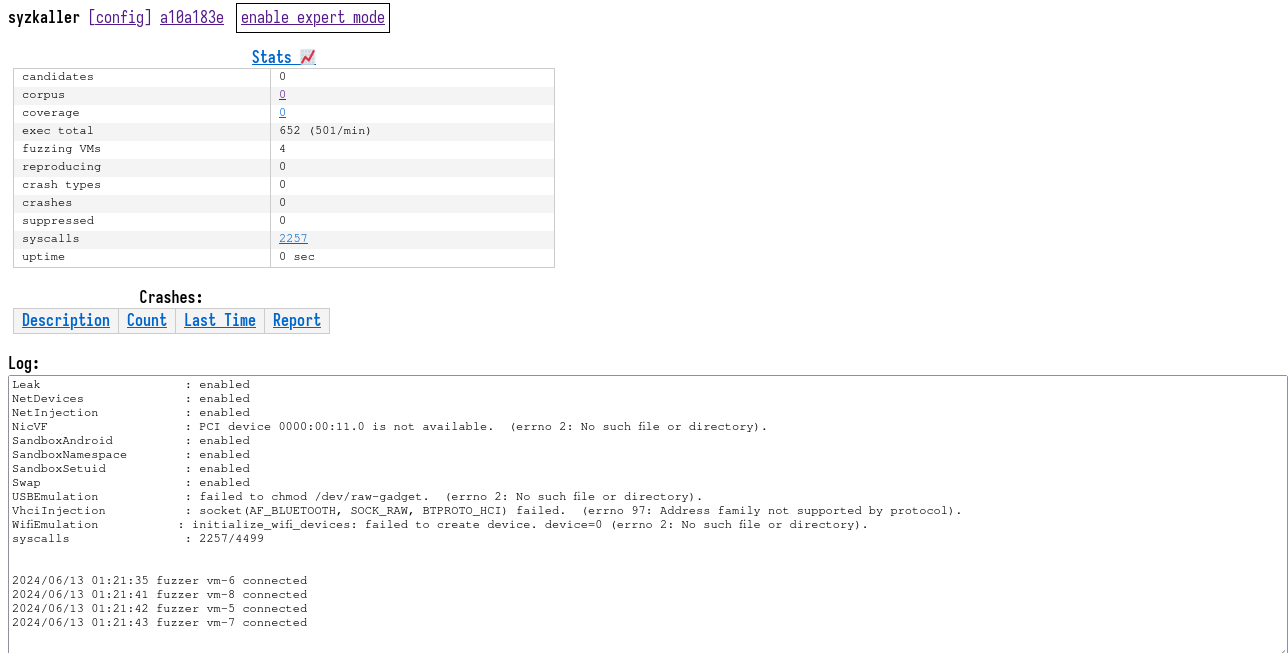
\includegraphics[width=0.95\textwidth]{figures/syzkaller-dashboard.png}
  \end{center}
  \caption{Esecuzione syzkaller}\label{fig:syz-dashboard}
\end{figure}

\clearpage
\section{IPsec}
IPsec (Internet Protocol Security) è una suite di protocolli per la protezione delle
comunicazioni IP attraverso l'autenticazione e la crittografia di ogni pacchetto IP in una
sessione. La suite contiene due protocolli principali:
\begin{itemize}
  \item Encapsulating Security Payload: è un protocollo che fa parte del framework IPsec 
    che incapsula il pacchetto originale e lo cripta. Consente di implementare la
    riservatezza dei dati, l'autenticazione della sorgente che la verifica dell'integrità
  \item Authentication Header: header che fornisce l'integratà dei dati e autenticazione 
    dell'origine, ma non offre funzioni di cifratura;
\end{itemize}

In particolare, IPsec ha due modalità di funzionanemto:
\begin{itemize}
  \item Transport mode: protegge solo il payload del pacchetto IP lasciando intatti gli 
    header originali;
  \item Tunnel mode: protegge l'intero pacchetto IP, incapsulandolo in un nuovo pacchetto IP
    con nuovi header;
\end{itemize}

\begin{figure}[h]
  \begin{center}
    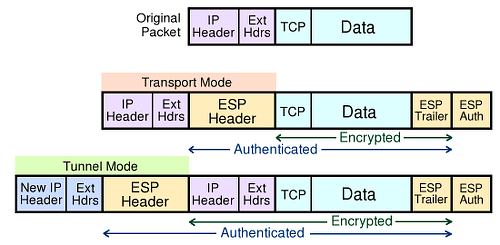
\includegraphics[width=.8\textwidth]{figures/esp-packet.png}
  \end{center}
  \caption{Struttura di un pacchetto ESP in tunnel e in transport mode}\label{fig:esp-packet}
\end{figure}

La componente principale di IPsec è la \textbf{\textit{Security Association (SA)}}: 
una connessione logica unidirezionale tra due host caratterizzata da:
\begin{itemize}
  \item SPI: stringa che identifica la security association locale;
  \item Indirizzo IP di destinazione: indirizzo della destinazione della SA;
  \item SPI: identifica se l'associazione SA è un Authentication Header o un 
      Encapsulation
\end{itemize}
Le SA sono conservate all'interno del \textbf{\textit{Security Association Database}} (SAD).

Infine, un componente fondamentale per IPsec è la gestione e lo scambio delle chiavi che 
avviene attraverso il protocollo \textbf{\textit{Internet Key Exchange}}.

\subsection{Implementazione IPsec in Linux}
Linux implementa in kernel space le strutture dati necessarie ad IPsec. In particolare,
in questo progetto, ci si soffermerà sul protocollo ESP in transport mode. In questo modo,
possono essere testati i componenti mostrati in \cref{fig:ipsec-linux}

\begin{figure}
  \begin{center}
    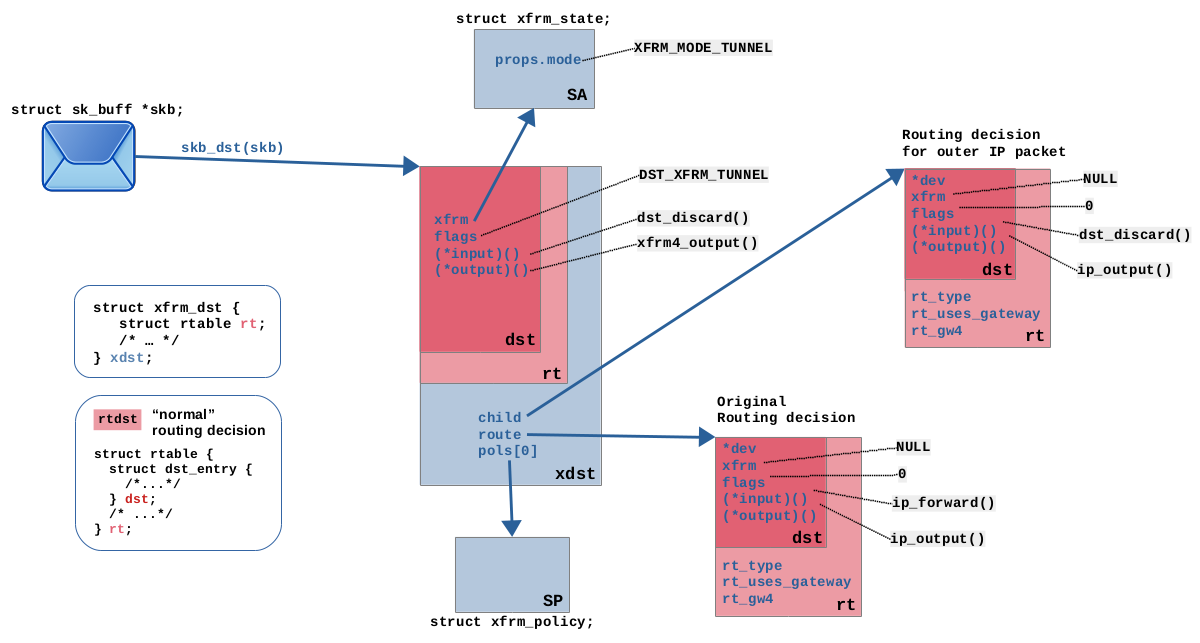
\includegraphics[width=0.95\textwidth]{figures/ipsec-linux.png}
  \end{center}
  \caption{Architettura IPsec in Linux}\label{fig:ipsec-linux}
\end{figure}


Dallo user space 
è possibile creare security association e manipolare i pacchetti IP in un particolare 
indirizzo con l'utility \textbf{\textit{ip xfrm}}. In particolare, dati due host 
tra i quali si vuole definire un canale sicuro, definite le 
seguenti variabili:

\begin{verbatim}
$ host1="IP_HOST_1"
$ host2="IP_HOST_2"
$ key12=0x$(xxd -c 32 -l 32 -ps /dev/random)
$ key21=0x$(xxd -c 32 -l 32 -ps /dev/random)
$ spi12=0x$(xxd -c 4 -l 4 -ps /dev/random)
$ spi21=0x$(xxd -c 4 -l 4 -ps /dev/random)
\end{verbatim}

È possibile creare una SA su entrambi gli host specificando modalità transport con protocollo 
ESP utilizzando AES come algoritmo di crittografia con i comandi:

\begin{verbatim}
$ ip xfrm state add src $host1 dst $host2 \ 
  proto esp spi $spi12 enc 'cbc(aes)' \  
  $key12 mode transport

$ ip xfrm state add src $host2 dst $host1 \ 
  proto esp spi $spi21 enc 'cbc(aes)' \ 
  $key21 mode transport
\end{verbatim}

Essendo le SA unidirezionali, esse vanno create in tutti i versi in cui si vuole che la 
comunicazione avvenga.

Successivamente, bisogna definire le security policy in cui si indica quali sono 
gli estremi della comunicazione modificando le strutture della tabella netfilter
(\cref{fig:packetflow-esp})
Ad esempio, sull'host1 bisogna configurare come in uscita il traffico in direzione 
host2 e viceversa (bisogna fare l'operazione duale sull'host2).
\begin{verbatim}
$ ip xfrm policy add dir out \
  src $host1 dst $host2 \ 
  tmpl proto esp mode transport

$ ip xfrm policy add dir in \ 
  src $host2 dst $host1 \ 
  tmpl proto esp mode transport
\end{verbatim}

\begin{figure}[h]
  \begin{center}
    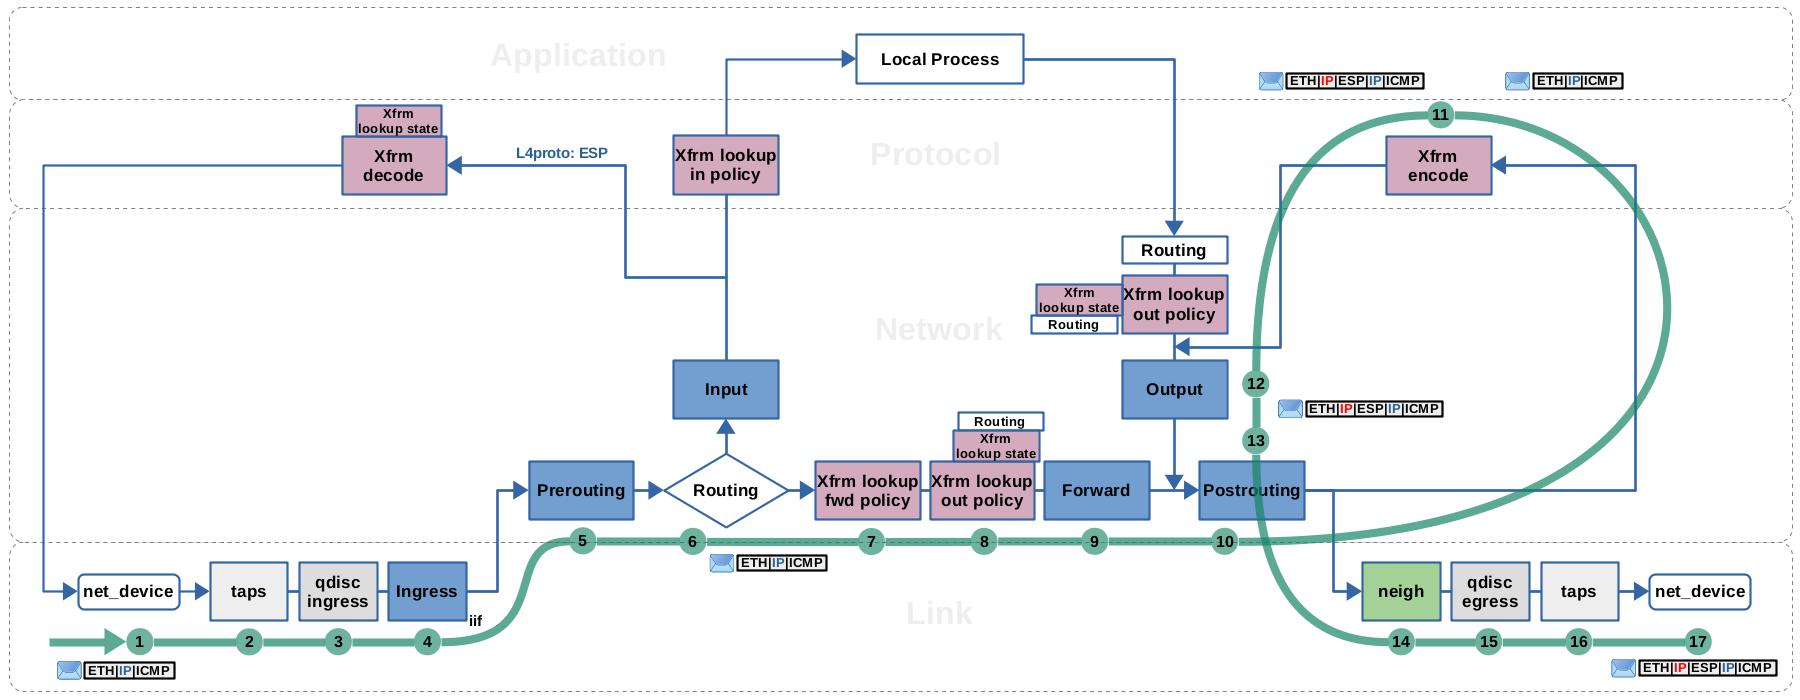
\includegraphics[width=0.95\textwidth]{figures/packet-flow-ipsec-tunnel-encrypt.png}
  \end{center}
  \caption{Flusso completo seguito da un pacchetto IPsec all'interno del kernel Linux}\label{fig:packetflow-esp}
\end{figure}


\clearpage
\section{Ambiente di test}
La difficoltà principale per il testing di IPsec è la creazione di un tunnel locale alla 
macchina virtuale. Il requisito principale è quello di generare traffico cifrato andando 
a coprire l'implementazione del protocollo IPsec all'interno del kernel. La figura in 
\cref{fig:basic-idea}
mostra la soluzione progettata.

\begin{figure}[h]
  \begin{center}
    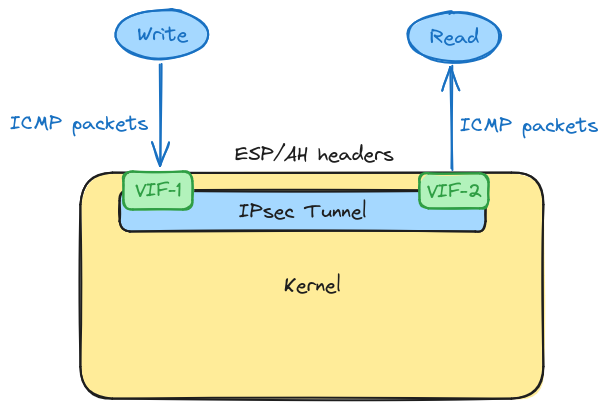
\includegraphics[width=.7\textwidth]{figures/basic-idea.png}
  \end{center}
  \caption{IPsec tunnel con interfacce virtuali}\label{fig:basic-idea}
\end{figure}
Infatti, a differenza di quanto mostrato in \cite{SyzkallerExternalNetworking}, in 
questo caso è necessario creare una comunicazione quanto più vicina alla realtà e utilizzando 
le interfacce TUN/TAP non è facile metterle in comunicazione.

\subsection{Approccio naive: interfacce TUN/TAP}
Il primo approccio tentato è quello della configurazione di una interfaccia TUN/TAP
\cite{LinuxDocs}. 
Questo tipo di interfaccia è già supportato in Syzkaller ed è di facile implementazione 
poichè consente di riutilizzare le procedure già definite per inviare pacchetti sull'interfaccia. 

La creazione della configurazione è mostrata in \cref{fig:tap-ipsec} e ripercorre quella già descritta in \cite{SyzkallerExternalNetworking}
aggiungendo come passaggio intermedio quello della configurazione delle SA sull'interfaccia.
In verde sono mostrate le funzionalità già implementate in \cite{SyzkallerExternalNetworking}

\begin{figure}
  \begin{center}
    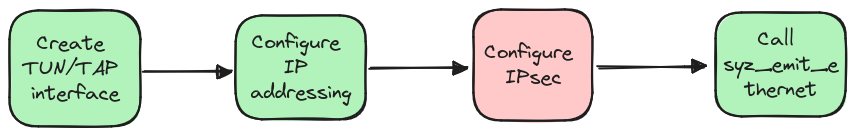
\includegraphics[width=0.95\textwidth]{figures/tap-ipsec.png}
  \end{center}
  \caption{Flusso configurazione IPsec su interfaccia TAP}\label{fig:tap-ipsec}
\end{figure}

\subsection{Approccio avanzato: network namespaces e virtual ethernet}
Una soluzione più completa prevede l'utilizzo del concetto di namespace all'interno del 
kernel Linux. In questo caso, sono stati utilizzati i \textbf{\textit{network namespaces}}
per creare ambienti di rete completamente isolati a cui è possibile aggiungere delle 
interfacce. 
Per la configurazione di test, è stato utilizzato il driver \textbf{\textit{veth}} del 
kernel linux che crea una coppia di interfacce virtuali ciascuna delle quali viene spostata 
nel suo namespace.

Come mostrato in \cref{fig:netns-config}, la  
configurazione implementata utilizza i network namespace per duplicare lo stack di rete 
implementato nel kernel.
\begin{figure}[h]
  \begin{center}
    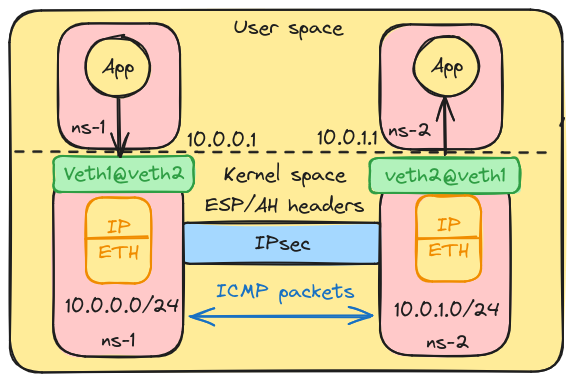
\includegraphics[width=.7\textwidth]{figures/netns-solution.png}
  \end{center}
  \caption{Configurazione con network namespaces}\label{fig:netns-config}
\end{figure}
Quest'approccio può essere vantaggioso per il fuzzing in quanto viene testata un'interfaccia più ampia che include:
\begin{itemize}
  \item le system call per la creazione di container: la creazione di un namespace Linux 
    include l'utilizzo delle system call di \textbf{\textit{unshare}}, \textbf{\textit{setns}} e 
    \textbf{\textit{clone}};
  \item implementazione del driver virtual ethernet;
  \item implementazione del sistema \textbf{\textit{xfrm}} per la manipolazione di pacchetti 
    IP;
\end{itemize}

Inoltre, configurando le interfacce per utilizzare IPsec possono essere utilizzate 
tutte le altre funzionalità già implementate in Syzkaller per il fuzzing delle funzionalità 
di rete (creazione socket TCP e UDP) senza implementare manualmente gli header ESP e AH.

\subsubsection{Configurazione}
Utilizzando una macchina di test, la configurazione è stata prodotta utilizzando semplici 
comandi da terminale che poi saranno tradotti in messaggi NETLINK, come spiegato di 
seguito e saranno utilizzate come pseudo-systemcall. Per creare un \textbf{\textit{network 
namespace}} si usa il comando:

\begin{verbatim}
$ ip netns add <ns-id> 
\end{verbatim}

Come qualsiasi namespace di Linux, supportano l'esecuzione di comandi al suo interno. Infatti, 
appena creato, il namespace contiene solo un'interfaccia di loopback (\cref{fig:netns-exec-iface}).

\begin{figure}[h]
  \begin{center}
    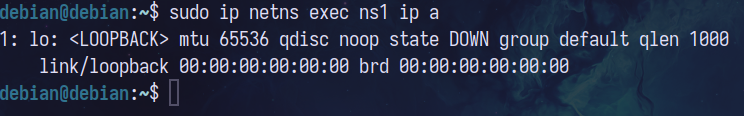
\includegraphics[width=0.95\textwidth]{figures/netns-exec-iface.png}
  \end{center}
  \caption{Interfacce presenti in un netns nuovo}\label{fig:netns-exec-iface}
\end{figure}

Successivamente si crea la coppia di interfacce virtuali, configura con gli indirizzi IP 
mostrati in \cref{fig:netns-config}, vengono
aggiunte ai namespace con il comando:

\begin{verbatim}
$ ip link add <veth-name-1> type veth peer name <veth-name-2>
$ ip link set <ifname> netns <netns-id>
\end{verbatim}

Quindi applicando anche la configurazione con \textbf{\textit{xfrm}}, si riesce ad avere 
un tunnel IPsec configurato come mostrato in \cref{fig:netns-esp}. 

\begin{figure}[h]
  \begin{center}
    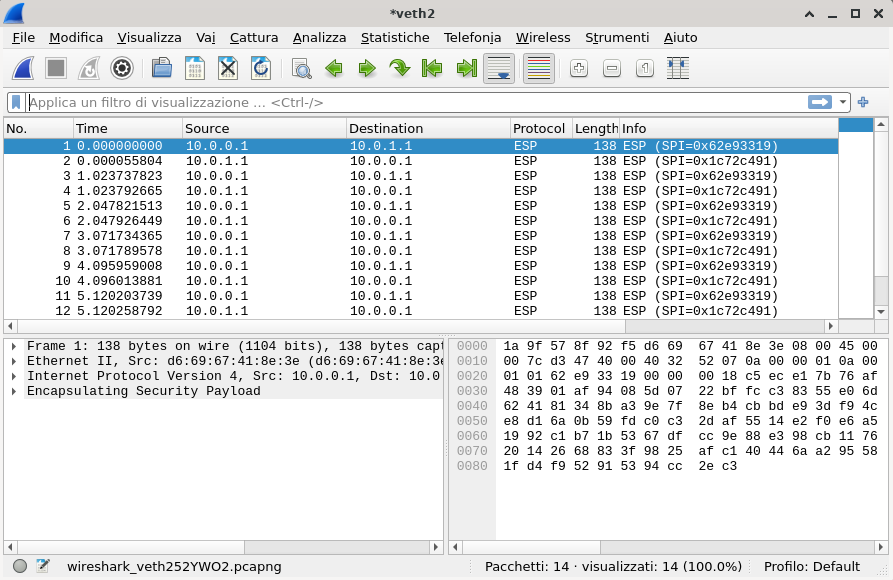
\includegraphics[width=.8\textwidth]{figures/netns-esp.png}
  \end{center}
  \caption{Realizzazione del tunnel IPSec tra network namespace separati}\label{fig:netns-esp}
\end{figure}

\subsection{Configurazione kernel: socket NETLINK}
Le socket NETLINK sono un meccanismo di comunicazione inter-processo (IPC) in Linux che 
permettono la comunicazione tra il kernel e gli utenti in spazio user. NETLINK viene utilizzato
per vari scopi, inclusi la configurazione della rete e la gestione delle politiche di 
sicurezza. All'interno del codice aggiunto a Syzkaller, le socket netlink sono utilizzate 
per configurare le interfacce di rete. Ad esempio, per aggiungere un'interfaccia ad 
un network namespace si può usare la funzione:

\begin{lstlisting}[language=C,caption=Migrazione di un'interfaccia di rete in un network namespace con messaggi Netlink in C]
// ip link set <ifname> netns <ns-id>
void move_if_to_pid_netns(char *ifname, int netns) {
    // gestione dell'errore omessa per brevità
    int sock_fd = socket(PF_NETLINK, SOCK_RAW | SOCK_CLOEXEC, NETLINK_ROUTE);

    struct nl_req req = {
            .n.nlmsg_len = NLMSG_LENGTH(sizeof(struct ifinfomsg)),
            .n.nlmsg_flags = NLM_F_REQUEST | NLM_F_ACK,
            .n.nlmsg_type = RTM_NEWLINK,
            .i.ifi_family = PF_NETLINK,
    };

    // funzioni di utlity per aggiungere parametri alla richiesta
    addattr_l(&req.n, sizeof(req), IFLA_NET_NS_FD, &netns, 4);
    addattr_l(&req.n, sizeof(req), IFLA_IFNAME,
              ifname, strlen(ifname) + 1);

    // invio del messaggio
    send_nlmsg(sock_fd, &req.n);

    close(sock_fd);
} 
\end{lstlisting}

Mentre invece per configurare una SA è stata usata una funzione simile alla seguente:

\begin{lstlisting}[language=C,caption=Creazione di una SA con socket Netlink in C]
void create_sa(int sock) {
    char buffer[NL_BUFSIZE];
    struct nlmsghdr *nlmsg = (struct nlmsghdr *)buffer;
    struct xfrm_usersa_info *sa_info;
    struct rtattr *rta;
    int key_len = 16;
    unsigned char key[16] = {0x00, 0x01, 0x02, 0x03, 0x04, 0x05, 0x06, 0x07, 
                             0x08, 0x09, 0x0A, 0x0B, 0x0C, 0x0D, 0x0E, 0x0F};

    memset(buffer, 0, NL_BUFSIZE);

    // Setup NLMSG header
    nlmsg->nlmsg_len = NLMSG_LENGTH(sizeof(struct xfrm_usersa_info));
    nlmsg->nlmsg_type = XFRM_MSG_NEWSA;
    nlmsg->nlmsg_flags = NLM_F_REQUEST | NLM_F_CREATE;
    nlmsg->nlmsg_seq = 1;

    // Setup SA info
    sa_info = NLMSG_DATA(nlmsg);
    sa_info->sel.family = AF_INET;
    inet_pton(AF_INET, "192.168.1.1", &sa_info->saddr);
    inet_pton(AF_INET, "192.168.1.2", &sa_info->id.daddr);
    sa_info->id.proto = IPPROTO_ESP;
    sa_info->id.spi = htonl(0x100);
    sa_info->lft.hard_byte_limit = XFRM_INF;
    sa_info->lft.hard_packet_limit = XFRM_INF;
    sa_info->lft.soft_byte_limit = XFRM_INF;
    sa_info->lft.soft_packet_limit = XFRM_INF;
    sa_info->mode = XFRM_MODE_TRANSPORT;
    sa_info->reqid = 0;

    // Add encryption key attribute
    rta = (struct rtattr *)((char *)nlmsg + NLMSG_ALIGN(nlmsg->nlmsg_len));
    rta->rta_type = XFRMA_ALG_CRYPT;
    rta->rta_len = RTA_LENGTH(sizeof(struct xfrm_algo) + key_len);

    struct xfrm_algo *alg = (struct xfrm_algo *)RTA_DATA(rta);
    strcpy(alg->alg_name, "cbc(aes)");
    alg->alg_key_len = key_len * 8;
    memcpy(alg->alg_key, key, key_len);

    nlmsg->nlmsg_len = NLMSG_ALIGN(nlmsg->nlmsg_len) + RTA_LENGTH(sizeof(struct xfrm_algo) + key_len);

    // Send Netlink message
    if (send_netlink_msg(sock, nlmsg) < 0) {
        perror("send_netlink_msg");
    }
}
 
\end{lstlisting}

\clearpage
\section{Implementazione in Syzkaller}
L'implementazione del fuzzing per IPsec prevede due fasi distinte derivanti dal fatto che 
il protocollo non include lo scambio delle chiavi e quindi si compone di due fasi distinte. 
Ciò può essere sfruttato per testare da due punti di vista differenti l'implementazione:
\begin{itemize}
  \item configurazione SA: utilizza lo strumento XFRM per creare delle entry all'interno 
    del SAD. Nella realtà, lo scambio e la gestione delle chiavi avviene con IKE e Diffie-Helman;
  \item generazione del traffico: invio di pacchetti con header IPsec;
\end{itemize}

\subsection{Fuzzing SA e SAD}
Per il fuzzing del sistema di gestione delle chiavi sono state predisposte 2 pseudo systemcall:
\begin{itemize}
  \item \textbf{\textit{syz\_emit\_ipsec()}}: aggiunge delle SA per la comunicazione tra due IP prima di inviare il 
    pacchetto;
  \item \textbf{\textit{syz\_flush\_ipsec()}}: elimina lo stato delle SA;
  \item \textbf{\textit{syz\_send\_ipsec()}}: encapsula un pacchetto IP in un header ESP;
\end{itemize}

Per forzare la creazione di stati incosistenti, la funzione flush è stata implementata 
come mostrato di seguito. 

\begin{lstlisting}[language=C,caption=Pseudo systemcall per la rimozione di SA dal SAD]
static long syz_flush_ipsec(volatile long a0) {
	int n = (int)a0;
	if (n < 0) {
		flush_ipsec_policy();
	} else if (n == 0) {
		flush_ipsec_policy();
		flush_ipsec_state();
	} else {
		flush_ipsec_state();
	}
	return 0;
}
\end{lstlisting}

Mentre la funzione \textbf{\textit{syz\_emit\_ipsec()}}, estrae gli indirizzi IP dalla frame 
e crea una SA per la coppia. In versione semplificata, la funzione è mostrata di seguito.
\begin{lstlisting}[language=C,caption=Creazione di una SA per una frame Ethernet]
static long syz_emit_ipsec(volatile long a0, volatile long a1, volatile long a2) {
  // controllo degli errori omessi
  struct ethhdr* eth = (struct ethhdr*)data;
  struct iphdr* ip = (struct iphdr*)(data + sizeof(struct ethhdr));

  // estrazione IP
  inet_ntop(AF_INET, &ip->saddr, src_ip, INET_ADDRSTRLEN);
  inet_ntop(AF_INET, &ip->daddr, dst_ip, INET_ADDRSTRLEN);

	add_ipsec_state(sock, src_ip, dst_ip, key, spi);
	add_ipsec_policy_out(sock, src_ip, dst_ip);
	add_ipsec_policy_in(sock, dst_ip, src_ip);

	return write(ipsec_tun, data, length);
}
\end{lstlisting}

Infine, è stata aggiunta una pseudo-systemcall per generare header ESP e incapsulare pacchetti. 
\begin{lstlisting}[language=C,caption=Incapsulamento di un pacchetto proveniente da una socket]
static long syz_send_ipsec(volatile long a0, volatile long a1, volatile long a2) {
  int sock = (int)a0;
	int length = (int)a2;
	uint8_t* data = (uint8_t*)a0;
	uint8_t* esp = 0;
	size_t* len = 0;
	int err;

	err = encapsulate_ip_in_esp(data, length, esp, len);

	if (err < 0)
		return err;

	return write(sock, esp, *len);
}
\end{lstlisting}



\subsection{Fuzzing header ESP e AH} 
Per testare l'handling di questi pacchetti è stata aggiunta la definizione di queste 
intestazioni per il protocollo IPsec nel file \textbf{vnet.txt}. Ad esempio, per 
esp:
\begin{verbatim}

esp_header {
	spi	int32be[0x1234:0x12345]
	seq	const[0x1, int32be]
	icv	int32[0x0:0xffffffff]
} [packed]

esp_trailer {
	pad_length	int8[0x0:0xff]
	next_header	const[ipv4_types, int8]
} [packed]

esp_packet {
	esp_hdr	esp_header
	data	ipv4_packet_t[flags[ipv4_types, int8], array[int8]]
	esp_tr	esp_trailer
} [packed]
\end{verbatim}
In questa definizione si definisce l'incapsulamento di un pacchetto IP con quanto 
viene specificato nella specifica di ESP. Infatti, \textbf{\textit{esp\_packet}} viene 
poi riportato all'interno dei pacchetti \textbf{\textit{ipv4}} definiti di seguito:

\begin{verbatim}
ipv4_packet [
  # ... altri tipi di pacchetti
	esp	ipv4_packet_t[const[IPPROTO_ESP, int8], esp_packet]
  # ... altri tipi di pacchetti
] [varlen] 
\end{verbatim}

Allo stesso modo, è stato aggiunto il supporto per \textbf{\textit{Authentication Header}}
sfruttando la possibilità di \textbf{\textit{syzlang}} di aggiungere campi con lunghezza
calcolata a runtime. Infatti, il campo \textbf{\textit{payload\_len}} viene calcolato con
la \textbf{\textit{macro}} che si riferisce alla lunghezza del pacchetto.

\begin{verbatim}
ah_header {
	next_header	const[ipv4_types, int8]
	payload_len	len[ah_header, int8]
	reserved	const[0x0, int16be]
	spi		int32be[0x1234:0x12345]
	seq		const[0x1, int32be]
	icv		int32[0x0:0xffffffff]
} [packed]

ah_packet {
	header	ah_header
	payload	ipv4_packet_t[flags[ipv4_types, int8], array[int8]]
} [packed]
\end{verbatim}

Infine, è stato aggiunto al tipologia di pacchetti supportati:
\begin{verbatim}
ipv4_packet [
  # altri pacchetti
	ah	ipv4_packet_t[const[IPPROTO_AH, int8], ah_packet]
] [varlen]
\end{verbatim}

\subsection{Esperimento}
Per cercare di focalizzare il testing sul sottosistema di rete, è stato avviato il fuzzing 
solo con le system call che possono impattare sulle strutture mostrate in 
\cref{fig:ipsec-linux} e \cref{fig:packetflow-esp} 
includendo la seguente lista nella configurazione:

\begin{verbatim}
// elenco abbreviato
"enable_syscalls": [
  "syz_emit_ethernet",
  "syz_emit_ipsec",
	"syz_send_ipsec",
	"syz_flush_ipsec",
	"syz_extract_tcp_res",
	"syz_extract_tcp_res$synack",
  "sendmsg$nl_xfrm",
  "socket$nl_xfrm",
	"socket$nl_netfilter",
	"socket$inet_icmp",
	"sendto",
	"recvfrom",
	"sendmsg",
	"recvmsg",
	"socket$igmp",
	"listen",
	"shutdown"
	] 
\end{verbatim}

In \cref{fig:corpus}, è mostrato un 
insieme di programmi generato dal sistema ordinati per coverage.
\begin{figure}[h]
  \begin{center}
    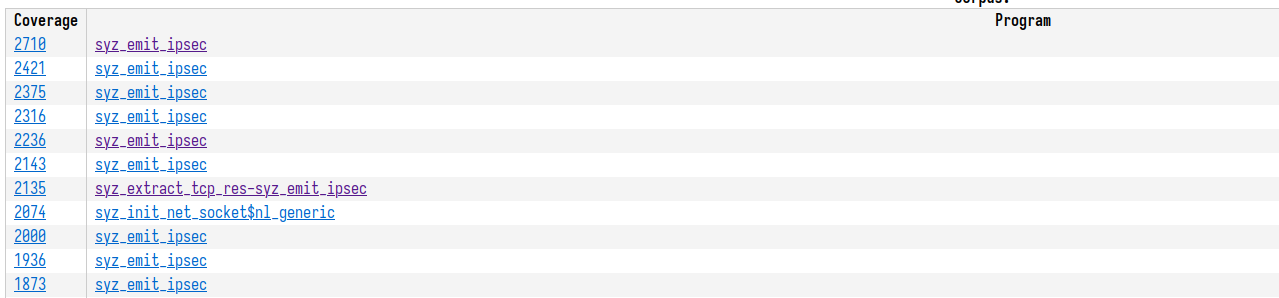
\includegraphics[width=.9\textwidth]{figures/corpus.png}
  \end{center}
  \caption{Programmi generati durante l'esecuzione}\label{fig:corpus}
\end{figure}

In \cref{fig:fuzzing}, è
riportata la dashboard di ricapitolazione del fuzzing.
\begin{figure}[h]
  \begin{center}
    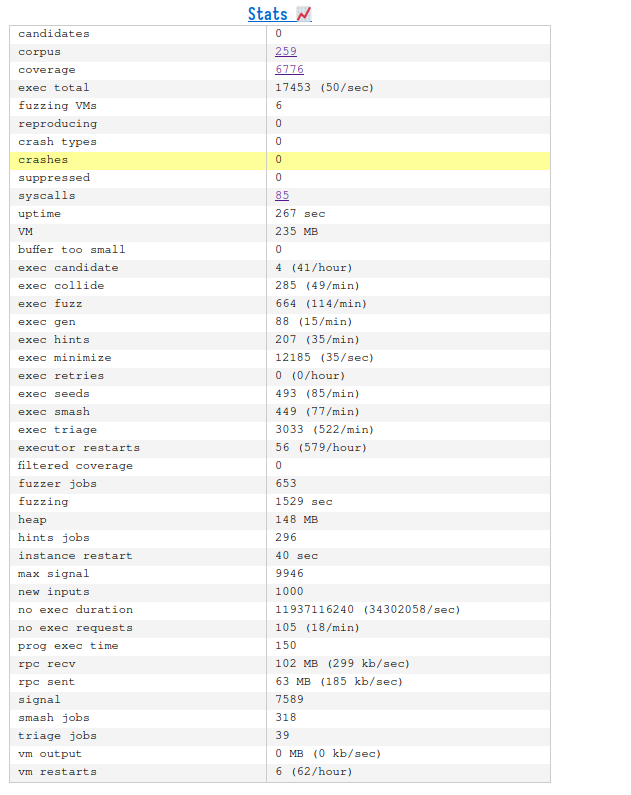
\includegraphics[width=.7\textwidth]{figures/experiment.png}
  \end{center}
  \caption{Esecuzione del fuzzing per il sottosistema di rete}\label{fig:fuzzing}
\end{figure}

In \cref{fig:coverage}, 
è mostrata la coverage raggiunta per il sottosistema \textbf{\textit{xfrm}} dopo alcuni minuti di 
esecuzione.

\begin{figure}
  \begin{center}
    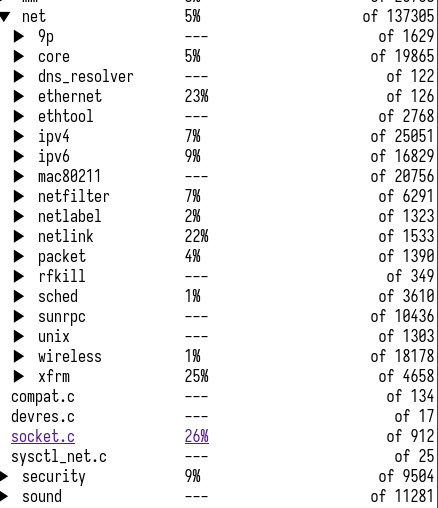
\includegraphics[width=0.95\textwidth]{figures/xfrm-coverage.png}
  \end{center}
  \caption{Coverage raggiunta del sistema XFRM dopo alcuni minuti di esecuzione}\label{fig:coverage}
\end{figure}


\clearpage
\bibliography{refs}
\bibliographystyle{apacite}

\end{document}
